\chapter{C}

\section{C语言的内存分配}
auto关键字修饰的变量,其申请的内存放在栈当中

register关键字修饰的变量,其申请的内存放在寄存器当中,并不是在内存当中,而是在cpu的
缓存当中,其访问速度比较快,常用于定义一些快速访问的变量。但是,cpu只是会尽量将这些
变量放在寄存器当中,如果寄存器不够了,还是会放在内存当中。另外,针对register修饰的变量
进行取地址操作是不起作用的。原因在于cpu的寄存器无法取地址。

对于内存的地址的分配的内容,可以使用unsigned char类型的指针进行查看。
\begin{code-block}{c}
void test()
{
    float a = 1.4;
    unsigned int *pointer_int;
    unsigned char * pointer_char;
    pointer_int = &a;
    pointer_char = &a; // float a为4字节的数据,pointer_char指向的数据为1字节的数据
                       // *pointer_char表示的是float a的16进制的最后2位
    printf("pointer_int is %x\n", *pointer_int);
    printf("pointer_char is %x\n", *pointer_char);
}
\end{code-block}

变量的内存分配是从高地址从低地址进行分配。
\begin{code-block}{c}
void test()
{
    int a = 0x1234567;
    unsigned char *p = (unsigned char*)&a; //每次读取一个字节
    // 在intel的cpu上,其输出结果基本如下:
    // The p is 67 and p+1 is 45, p+2 is 23, and p+3 is 1
    printf("The p is %x and p+1 is %x, p+2 is %x, and p+3 is %x\n", *p, *(p+1), *(p+2), *(p+3));
    return 0;
}
\end{code-block}

利用这种分配特性,我们可以通过指针进行越界访问,操作其他变量的值。
\begin{code-block}{c}
void test()
{
    const int first = 1; //假设first的地址为0xf4
    int second = 2;      //则second的地址为0xf0。注意,只要是这样连续定义,变量的地址一定是连续的。
    printf("%p\t%p\n", &first, &second);
    int *pointer_int = &second;
    *(pointer_int+1) = 100; //pointer_int+1指向了first的地址
                            // 通过这种越界访问的方式,则访问并修改了first的值。
    printf("%d\n", first);
}
\end{code-block}

从总体内存分布当中来看,C语言的内存分配存在如下的特点:
\begin{itemize}
  \item 代码段放在内存的低地址当中,通常是放在0x804或者0x40开头的低地址当中。代码段是静态地址。为只读的内存段
  \item 代码段上面则是只读数据段,存放不可变数据,比如字符串“hello world”就属于存放于该部分,这一部分也是只读的内存段
  \item 全局数据空间,即存放全局变量的地方。static修饰的数据也放在这部分(不管修饰的是全局的还是局部的变量)。
    如果只是用static修饰定义,但是没有赋初值,则对应的变量放在bss段,而不是data段。
    static int a = 100 ,a会放在data段,static int b;b则是放在bss段。这一部分为可读可写的内存。
    const修饰的变量并没有放到内存的只读区,同样是放在内存的可读可写区域
  \item 代码段上面则是运行时的堆地址,通常使用malloc,calloc或者realloc等函数所申请的空间地址
  \item 堆地址之上,则是栈地址,通常用于存放代码当中的临时变量
  \item 栈地址之上则是内核空间,这部分的地址则是应用程序无法访问的地方,也是禁止访问的地址
\end{itemize}

代码段,只读数据段,全局数据空间统称为静态数据段,在汇编的实现当中,代码段和只读数据段统称为text,而全局数据空间则称为data和bss(未初始化数据段)。
字符串数据放在text段。
通常情况下,可以使用size命令查看一个二进制文件的代码分布。如\nameref{fig:size}所示:
\begin{figure}[H]
  \centering
  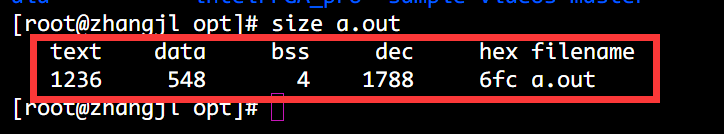
\includegraphics[scale=0.8]{size.png}
  \caption{内存分布}
  \label{fig:size}
\end{figure}

\begin{code-block}{c}
printf("hello world\n");

// 与上述代码对比
// printf("1234hello world\n"); 在编译生成的二进制文件当中,通过size命令可以
// 看到text段多出了4个字节
\end{code-block}

除此之外,C语言的函数实际上也是地址,我们可以通过地址,获得函数入口,进行调用。
\begin{code-block}{c}
int (*printfunc)(const char * ,...);
printfunc = (int (*)(const char *,...))0x400420; // 假设printf函数的内存地址为该数值
printfunc("hello world\n"); // 相当于调用printf("hello world \n");
\end{code-block}

\section{通用交换函数}
通用的交换函数(非字符串)
\begin{code-block}{c}
#include <stdlib.h>
#include <string.h>
void swap_object(void * first, void * last, size_t size)
{
    void * tmp = malloc(size);
    memcpy(tmp, first, size);
    memcpy(first, last, size);
    memcpy(last, tmp, size);
    free(tmp);
}
\end{code-block}

\section{柔性数组}
C语言的数据和python的不一样,是一个定长的,也就是说,需要预先设定好长度。如果需要
使用变长数组,则需要使用指针。通过指针的方式,一个一个的分配。但是,这种方式,不利于
计算数组长度,当需要使用数据长度时,就会出现问题。柔性数组则不一样,可以当成变长
数据使用,同时,还可以确定长度。

柔性数据的定义如下
\begin{code-block}{c}
typedef struct _soft_array * array_ptr;
typedef struct _soft_array{
    size_t lenth;
    int members[1];
}soft_array;
\end{code-block}

柔性数组一般由2部分组成,第一个表示数组长度,第二个表示数据的元素。但是,由于
各个c/c++编译器的不一致,第二个参数,一定要是一个数组,并且,最好这个数组的长度
为1。在gcc当中,这个members的长度可以为0,但在clang/virsual c++当中,则可能报错。
统一设置为1,则不会出现这个问题。

柔性数组的使用
\begin{code-block}{c}
array_ptr init_soft_array(size_t lenth){
    array_ptr arrays = NULL;
    if(NULL == (arrays = malloc(
        offsetof(soft_array, members) + sizeof(int) * lenth))){
        printf("Cannot allocate more memory\n");
        return NULL;
    }
    arrays->lenth = lenth;
    for(size_t index = 0; index < lenth; index++){
        arrays->members[index] = index;
    }
    return arrays;
}
\end{code-block}

\section{指向指针的指针}
指向指针的指针,通常用在需要改变指针的地方。常见的操作,就是使用指向指针的指针
来删除单链表。
\begin{code-block}{c}
void delete_link(nodeptr * header, nodeptr delete_node) {
    nodeptr * current = header;
    nodeptr entry = NULL;
    while(*current) {
        entry = *current;
        if(entry == delete_node) {
            *current = entry -> next;
            free(delete_node);
            delete_node= NULL;
            return;
        } else {
            current = &(entry->next);
        }
    }
}
\end{code-block}

\section{二叉树的简单实现}
通常的,二叉树都是有序的二叉树,因此,插入时,一般都应当对其进行排序操作。
\begin{code-block}{c}
typedef struct _tnode * tree;
typedef void (*visit_func)(tree * root);

typedef struct _tnode{
    tree leftchild;
    tree rightchild;
    int value;
}tnode;

void insert_tree(tree *root, int value){
    if(NULL == *root){
        *root = MALLOC(1, tnode);
        if(NULL == *root){
            printf("Cannot allocate more memory for tree\n");
            return;
        }
        (*root)->value = value;
        (*root)->leftchild = NULL;
        (*root)->rightchild = NULL;
        return;
    }
    if((*root)->value > value){
        insert_tree(&((*root)->leftchild), value);
    }else{
        insert_tree(&((*root)->rightchild), value);
    }
}
\end{code-block}

对于二叉树而言,最重要的操作莫过于遍历。所有的二叉树操作都是基于遍历进行的。
二叉树的遍历操作通常有3种:前序,中序和后序。其中,最重要的,就是后序遍历。

\begin{code-block}{c}
// 前序遍历
void visit_tree_root_first(tree root, visit_func visit){
    if(NULL == root){
        return;
    }
    visit(&root);
    visit_tree_root_first(root->leftchild, visit);
    visit_tree_root_first(root->rightchild, visit);
}

// 中序遍历
void visit_tree_root_second(tree root, visit_func visit){
    if(NULL == root){
        return;
    }
    visit_tree_root_second(root->leftchild, visit);
    visit(&root);
    visit_tree_root_second(root->rightchild, visit);
}

// 后续遍历
void visit_tree_root_last(tree *root, visit_func visit){
    if(NULL == *root){
        return;
    }
    visit_tree_root_last(&((*root)->leftchild), visit);
    visit_tree_root_last(&((*root)->rightchild), visit);
    visit(root);
}
\end{code-block}

二叉树其他的操作,基本上也是根据遍历操作来实现的。比如,一颗二叉树的销毁。
\begin{code-block}{c}
static void _destroy_tree(tree * root){
    (*root)->leftchild = NULL;
    (*root)->rightchild = NULL;
    free(*root);
    *root = NULL;
}

void destroy_tree(tree *root){
    visit_func visit = _destroy_tree;
    visit_tree_root_last(root, visit);
}
\end{code-block}

\section{宏定义的高级使用}
\begin{outline}[enumerate]

\1 使用typeof创建范型宏
\begin{code-in-enumerate}{c}
#define MIN(x, y) ({                \
    typeof(x) _min1 = (x);          \
    typeof(y) _min2 = (y);          \
    (void) (&_min1 == &_min2);      \
    _min1 < _min2 ? _min1 : _min2; })
\end{code-in-enumerate}
但是,如果在编译的时候,使用了-std和-ansi参数,则上面的宏会失效。需要对他做部分的修改。
\begin{code-in-enumerate}{c}
#define MIN(x, y) ({                    \
    __typeof__(x) _min1 = (x);          \
    __typeof__(y) _min2 = (y);          \
    (void) (&_min1 == &_min2);          \
    _min1 < _min2 ? _min1 : _min2; })
\end{code-in-enumerate}
另外,使用-std和-ansi参数的时候,typeof需要替换为\_\_typeof\_\_, asm需要替换为
\_\_asm\_\_,inline也需要替换为\_\_inline\_\_。

\1 定义通用的错误处理
\begin{code-in-enumerate}{c}
#define errout(...) fprintf(stderr, "File %s Function %s Line %d ", \
        __FILE__, __FUNCTION__, __LINE__);                          \
        fprintf(stderr, ##__VA_ARGS__)
int main(int argc, char * argv[])
{
    errout("swap_object function %d\n", 123);
    errout("swap_object function\n");
    return 0;
}
\end{code-in-enumerate}

\1 使用\#\#连接不同的标识符
\begin{code-in-enumerate}{c}
#define appendidentify(first, last) first##last
int main(int argc, char * argv[])
{
    char * first = "lucifer";
    char * last = "garuda";
    char * firstlast = "let`s go";
    printf("%s\n", appendidentify(first, last));
    // 实际上相当与 printf("%s\n", firstlast);
    return 0;
}
\end{code-in-enumerate}

\1 将变量名称转换为字符串
\begin{code-in-enumerate}{c}
#define NAME_TO_STRING(name) (#name)
int main(int argc, char * argv[])
{
    char * firstlast = "let`s go";
    // 输出结果为"firstlast"
    printf("%s\n", NAME_TO_STRING(firstlast));
    return 0;
}
\end{code-in-enumerate}

\1 使用宏定义修改函数入口
\begin{code-in-enumerate}{c}
#ifdef CONFIG_SDL
int qemu_main(int argc, char **argv, char **envp);

int main(int argc, char **argv)
{
    printf("hello main with 2 params\n");
    return qemu_main(argc, argv, NULL);
}
#undef main
#define main qemu_main
#endif

int main(int argc, char **argv, char **envp)
{
    printf("main with envp\n");
    return 0;
}
\end{code-in-enumerate}
由于main方法可以接收多个参数,因此上述代码是正确合法的。现在简单的分析一下。
分析的手法是直接使用gcc -E参数来观察预处理的结果。

不添加CONFIG\_SDL宏,其结果是:
\begin{code-in-enumerate}{bash}
gcc -E test.c
int main(int argc, char **argv, char **envp)
{
    printf("main with envp\n");
    return 0;
}
\end{code-in-enumerate}
添加CONFIG\_SDL宏,其结果是:
\begin{code-in-enumerate}{bash}
gcc -E -D CONFIG_SDL test.c
int qemu_main(int argc, char **argv, char **envp);
int main(int argc, char **argv)
{
    printf("hello main with 2 params\n");
    return qemu_main(argc, argv, ((void *)0));
}

int qemu_main(int argc, char **argv, char **envp)
{
    printf("main with envp\n");
    return 0;
}
\end{code-in-enumerate}
从代码中可以看到,实际上,整个处理过程中通过undefine main和define main qemu\_main
这2条语句,就直接修改了整个操作的入口。实际上,这个代码的核心,就是将函数名当作
了一个宏定义,通过简单的名称替换,达到更改程序入口的目的。以上代码的用法,在qemu的
源码vl.c代码当中。

\1 获取结构体的数据偏移量
\begin{code-in-enumerate}{c}
#define offsetof(TYPE, MEMBER) ((size_t) &((TYPE *)0)->MEMBER)
typedef struct user user;
struct user{
    char * name;
    uint8_t age;
    //uint8_t age:7; 表示只占用该数据类型的最后7 bit,也就是说限制age不能大于127
    user* prev;
    user* next;
};

int main(int argc, char * argv[])
{
    printf("%ld\n",offsetof(user, name));
    printf("%ld\n",offsetof(user, prev));
    printf("%ld\n",offsetof(user, next));
    return 0;
}
\end{code-in-enumerate}

在((TYPE *)0)->MEMBER)这个其实就是提取type类型中的member成员,那么\&((TYPE *)0)->MEMBER)
得到member成员的地址,再强制转换成size\_t类型(unsigned int)。
但是这个地址很特别,因为TYPE类型是从0x0开始定义的,那么我们现在得到的这个地址就是
member成员在TYPE数据类型中的偏移量。这个宏定义的效果和c库当中的offsetof(stddef.h)功能一样。
以上的代码当中,输出的结果是0,8,16和24(64位平台)。原因是每一个指针的大小固定为
平台的位数,64位为8字节,32位为4字节。

需要注意的是,如果结构体成员当中存在 uint8\_t age:7 这种位成员时,是不能通过offsetof
获取age这种位成员的地址偏移量的。另外,所有对这种位成员进行取地址的操作,都是非法的。

\1 根据偏移量获取数据地址
\begin{code-in-enumerate}{c}
#define container_of(ptr, type, member) ({                           \
        const typeof( ((type *)0)->member ) *__mptr = (ptr);         \
        (type *)( (char *)__mptr - offsetof(type,member) );})
#define list_entry(ptr, type, member)                                \
        container_of(ptr, type, member)
\end{code-in-enumerate}

const typeof(((type *)0)->member) *\_\_mptr = (ptr);首先将0转化成type类型的指针变量
(这个指针变量的地址为0x0),然后再引用member成员(对应就是((type *)0)->member ))。
注意这里的typeof(x),是返回x的数据类型,那么 typeof(((type *)0)->member)其实就是
返回member成员的数据类型。那么这条语句整体就是将\_\_mptr强制转换成member成员的数据类型,
再将ptr的赋给它(ptr本身就是指向member的指针)。offsetof得到的是member成员在TYPE数据类型
中的偏移量。 (type *)((char *)\_\_mptr – offsetof(type,member))求的就是type的地址,
即指向type的指针。不过这里要注意\_\_mptr被强制转换成了(char *),为何要这么做?
因为如果member是非char型的变量,比如为int型,并且假设返回值为offset,那么这样直接减去偏移量,
实际上\_\_mptr会减去sizeof(int)*offset!这一点和指针加一减一的原理相同。当然,char*指针可以
替换为void*指针,可能会更加通用。有了这个指针,那么就可以随意引用其内的成员了。关于container\_of
的第二行,其效果类似如下。通过这个测试代码,可以发现pos的值和zhangjl的地址的值是
一模一样的,因此,可以通过pos指针访问student zhangjl当中的所有数据。
\begin{code-in-enumerate}{c}
int main(int argc, char * argv[])
{
        LIST_HEAD(first);
        student zhangjl = {.name="zhangjl", .age=18, .order=head};
        student *pos;
        printf("%x\n", &zhangjl);
        printf("%x\n", &zhangjl.order);
        printf("%ld\n", offsetof(student, order));
        //printf("%x\n", (void * )&zhangjl.order - offsetof(student, order));
        printf("%x\n", (char * )&zhangjl.order - offsetof(student, order));
        pos = (student*)((void *)&zhangjl.order - offsetof(student, order));
        printf("%x\n", pos);
        return 0;
}
\end{code-in-enumerate}

具体使用可以参见下方完整代码。
\begin{code-in-enumerate}{c}
typedef struct list_head list_head;
struct list_head {
        list_head *next, *prev;
};

typedef struct student student;
struct student {
        char * name;
        int age;
        list_head order;
};

#define offsetof(TYPE, MEMBER) ((size_t) &((TYPE *)0)->MEMBER)

#define LIST_HEAD_INIT(name) { &(name), &(name) }
#define LIST_HEAD(name)                                              \
        list_head name = LIST_HEAD_INIT(name)

#define container_of(ptr, type, member) ({                           \
        const typeof( ((type *)0)->member ) *__mptr = (ptr);         \
        (type *)( (char *)__mptr - offsetof(type,member) );})

#define list_entry(ptr, type, member)                                \
        container_of(ptr, type, member)

#define list_for_each_entry(pos, head, member)                       \
        for (pos = list_entry((head)->next, typeof(*pos), member);   \
            &pos->member != (head);                                  \
            pos = list_entry(pos->member.next, typeof(*pos), member))

static inline void __list_add(list_head *_new,
                list_head *prev, list_head *next)
{
        next->prev = _new;
        _new->next = next;
        _new->prev = prev;
        prev->next = _new;
}

static inline void list_add_tail(list_head *_new, list_head *head)
{
        __list_add(_new, head->prev, head);
}

int main(int argc, char * argv[])
{
        LIST_HEAD(head);
        student zhangjl = {.name="zhangjl", .age=18, .order=head};
        //student luoyan = {.name="luoyan", .age=18, .order=first};
        student luoyan = {.name="luoyan", .age=18, .order=LIST_HEAD_INIT(luoyan.order)};
        list_add_tail(&(luoyan.order), &(zhangjl.order));

        student *pos;

        list_for_each_entry(pos, &head, order){
        //list_for_each_entry(pos, &zhangjl.order, order){
                printf("%ld\n", pos);
                printf("%s\n", pos->name);
        }

        return 0;
}
\end{code-in-enumerate}

\1 发现编译时的错误

Linux 内核当中存在2个非常特殊的宏定义,如下:
\begin{code-in-enumerate}{c}
#define BUILD_BUG_ON(condition) ((void)sizeof(char[1 - 2*!!(condition)]))
#define BUILD_BUG_ON_ZERO(e) (sizeof(struct { int:-!!(e); }))
\end{code-in-enumerate}

下面对于上述的宏定义,进行简单的讲解:
\begin{enumerate}
  \item !!表示将e的结果连续取反,得到0或者1
  \item char[1-2*0]为合法结果,但是,char[1-2*1]为非法结果
  \item struct的位域定义当中,int:1 表示定义了一个匿名的位域空间,占据1位,int:0表示占据0位,int:-1则为非法表达式
\end{enumerate}

\end{outline}

\section{匿名结构体}
在定义结构体时,可以嵌入一个另外的结构体
\begin{code-block}{c}
typedef struct _user {
    char * name;
    uint8_t age;
    struct {
        char * child_name;
        uint8_t child_age;
    };
}user_struct;

int main(int argc, char * argv[])
{
    user user_ptra = malloc(sizeof(user_struct));
    user_ptra -> age = 20;
    user_ptra -> name = "zhangjl";
    user_ptra -> child_name = "zhangzz";
    user_ptra -> child_age = 18;
    printf("%s\t%d ==> %s\t%d\n", user_ptra -> name, user_ptra -> age,
           user_ptra -> child_name, user_ptra -> child_age);
    return 0;
}
\end{code-block}

\section{位移运算}
\begin{code-block}{c}
// 设置某一位为高电平(1),其余位不变
a = a | (0x1<<n)
a |= (0x1<<n)

// 设置某一位为低电平(0),其余位不变
a &= (~(0x1<<n))
\end{code-block}
